%Farid
\chapter{Présentation  Du Système }
\addcontentsline{toc}{chapter}{Présentation  Du Système }

 \section{Le Procède}

      Le procédé est le même que celui qui a été utilisé dans le TP du module I4 intitulé "Modélisation, analyse et com-mande d’une distribution hydraulique à trois bacs d’eau". Nous redonnons ici les caractéristiques essentielles de la manipulation.
      
\begin{center}
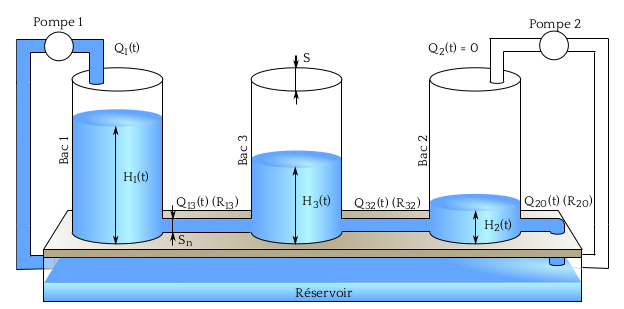
\includegraphics[scale=0.5]{fig1.png}
\captionof{figure}{\textit{ Procédé trois bacs.\cite{ref1}}}
\label{fig1} 
\end{center}

      Le système représenté sur la Figure 2.1 est composé de trois bacs cylindriques en plexiglas de section S. Ces trois bacs sont disposés en série (de gauche à droite, on trouve les bacs 1, 3 et 2) et sont reliés par des tuyaux d’écoulement de section S n .
      
      Le dernier bac 2 se vide par un cylindre, également de section S n , dans le réservoir situé sous les bacs. Deux pompes de débit Q 1 (t) et Q 2 (t) permettent de remplir respectivement les bacs 1 et 2 avec l’eau récupérée dans le réservoir, le système fonctionnant en circuit fermé.

      Les valeurs données par le constructeur sont S = 0, 0154m 2 et S n = 5.10 –5 m 2 .
      Les pompes obéissent à la relation V qi (t) = k · Q i (t) + b, i = 1, 2, avec k = 1, 6.10 5 et b = –9, 2592; où V qi et Q i (t) représentent respectivement la tension appliquée à la pompe i et le débit correspondant.
      Les pompes sont alimentées par une tension comprise entre [–10V, 10V]. Ainsi le débit maximal, Q max
délivrée par une pompe est 12.10 –5 m 3 /s lorsque la tension appliquée est de +10V. Les capteurs de niveau d’eau sont supposés linéaires autour du point de fonctionnement. Leur caractéristique est modélisé par l’équation H i (t) = k i · V h i (t) + b i , où H i est exprimé en mètres.\cite{ref1}


 \section{Le Modèle Linéarisé }
 
      Nous considérons le procédé actionné par la seule pompe numéro 1. Son débit Q 1 est compris entre [0, Q max ] suivant sa tension d’alimentation; le débit Q 2 (t) délivré par la pompe 2 sera nul tout au long de la manipulation. Ainsi, les différentes hauteurs H 1 (t), H 3 (t) et H 3 (t) respectent par conséquent la condition H{1}(t)$\geq$H{3}(t)$\geq$H{2}(t).\\ 
      La seule mesure disponible lors de cette manipulation est la mesure de la hauteur d’eau H 1 .\\
      
      Le travail sera réalisé sur un modèle aux faibles variations autour d’un point d’équilibre H 0 et d’un débit Q 10 à ce point d’équilibre de telle sorte que:

\begin{equation}
\left\{\begin{matrix}
Q1(t)=q1(t) +Q10\\
H{1}(t)=h{1}(t) +H{10}\\
H{3}(t)=h{3}(t) +H{30}\\
H{2}(t)=h{2}(t) +H{20}\\
\end{matrix}\right.
\end{equation} 


$H{0}$=$\begin{bmatrix}
H{10}\\
H{20}\\
H{30}\\
\end{bmatrix}$
\quad=\quad
$\begin{bmatrix}
0.27474\\
0.0299\\
0.1368\\
\end{bmatrix}$\\\\

$Q{10}$=$3.5*10^{-5}$\\

Le modèle D’état est\\


$\dot{h}(t)$=$\begin{bmatrix}
-0.0092 & 0.0092 & 0 \\
0.0092 & -0.0198 & 0.0106\\
0 & 0.0106 & 0.0486\\
\end{bmatrix}h(t)
\quad+\quad
\begin{bmatrix}
64.9351\\
0\\
0\\
\end{bmatrix}q1(t)$\\\\\\
$y(t)$=$\begin{bmatrix}
1 & 0 & 0
\end{bmatrix}q1(t)$\\

 

